\chapter{Desarrollo de una interfaz gráfica de usuario}\label{capitulo_4}
Uno de los objetivos principales del presente trabajo es el desarrollo de una interfaz gráfica de usuario para el control centralizado de la prótesis híbrida planteada en el capítulo \ref{capitulo_1}. Con dicha interfaz se pretende manejar el exoesqueleto, hasta cuatro electroestimuladores así como el conjunto de sensores necesarios.
\\
\\
Este control se efectúa de forma inalámbrica: en primer lugar, la interfaz gráfica establece comunicación con el módulo Bluetooth Sparkfun Silver mencionado en el capítulo \ref{capitulo_2}. A continuación, éste sirve como intermediario para la comunicación entre la interfaz gráfica y la prótesis híbrida, la cual se lleva a cabo mediante los protocolos de comunicación descritos en el capítulo \ref{capitulo_3}.
\\
\\
En el presente capítulo se va a exponer cómo se ha desarrollado la interfaz además de sus características, funcionalidades, capacidades y limitaciones.

\section{Entorno de desarrollo y herramientas}
El entorno de desarrollo elegido para esta aplicación es Visual Studio Code y el lenguaje de programación Python3. El autor del presente trabajo ha elegido dicho entorno de desarrollo porque además de ser gratuito, otorga una gran facilidad a la hora de integrar paquetes y bibliotecas. Además,  presenta una interfaz clara y fácil de utilizar incluso en el desarrollo de proyectos de cierta envergadura. En cuanto al lenguaje de programación, el autor ha seleccionado Python por su flexibilidad, sencillez y la gran cantidad de librerías disponibles para la integración de diferentes herramientas y funcionalidades. Es más, se detallan a continuación todas las necesarias para el desarrollo de esta interfaz:
\begin{itemize}
\item[•] \textbf{tkinter, ttk:} se trata del conjunto de herramientas para el desarrollo de interfaces gráficas que permite crear ventanas que recogen el conjunto de widgets (botones, entradas de texto, listas desplegables etc.) y demás elementos gráficos que dan forma a una interfaz gráfica de usuario.
\item[•] \textbf{pyserial:} es la librería que permite manejar herramientas de comunicación por puerto serie que en este caso se utilizan para la comunicación entre la interfaz y el módulo Bluetooth mencionado en el capítulo \ref{capitulo_2}.
\item[•] \textbf{threading:} la interfaz que se pretende elaborar debe realizar un número considerable de tareas no solamente en paralelo sino en tiempo real. Esto implica la necesidad de tener la capacidad de crear hilos de procesamiento para cumplir con la ejecución de todas las tareas estipuladas.
\item[•] \textbf{matplotlib:} para la creación de gráficos en los que mostrar datos relevantes durante la sesión de rehabilitación. Por ejemplo, es importante conocer las medidas de ángulos recibidas por los electrogoniómetros y/o exoesqueleto y que permiten apreciar, en una de sus diferentes formas, las etapas del ciclo de marcha.
\item[•] \textbf{numpy:} para el tratamiento rápido y eficaz de conjuntos extensos de datos.
\end{itemize}



\section{Integración de estimuladores}
Una de las capacidades de la mencionada interfaz de usuario es el control de hasta cuatro electroestimuladores. Se detalla a continuación el conjunto de funcionalidades que se desean implementar en la interfaz en cuanto al control de estos dispositivos se refiere:

\begin{itemize}
\item[•] Seleccionar el número de dispositivos que se van a utilizar.
\item[•] Establecer el valor de todos los parámetros de cada estimulador de manera correcta. Esto implica que estén dentro del rango de valores de corriente, ancho de pulso y frecuencia explicados en el capitulo anterior así como contrarrestar la conversión interna que el estimulador efectúa sobre dichos parámetros.
\item[•] Leer el valor de los parámetros ya configurados en el dispositivo.
\item[•] Guardar los valores de los parámetros configurados en la EEPROM del estimulador.
\item[•] Guardar y cargar todos los parámetros del mini TEREFES en un archivo de texto externo.
\item[•] Configurar el modo de operación de cada estimulador así como controlar el estado de su fuente de corriente (apagada o encendida) y el de la estimulación (iniciada o detenida).
\item[•] Como funcionalidad adicional, mostrar al usuario mensajes informativos y de posibles errores durante el uso de la interfaz.
\end{itemize} 

Una vez vistas las funcionalidades deseadas en la interfaz, se procede ahora a exponer ésta y cómo cumple con los objetivos mencionados. De este modo, la interfaz de usuario se compone de tres sectores principales: izquierdo, central y derecho, los cuales pueden apreciarse en la figura \ref{fig:interfaz}. Se recomienda disponer de esta imagen durante la lectura del resto de explicaciones referidas a la interfaz para su mejor comprensión.\\

\begin{figure}[!htb]
\centering
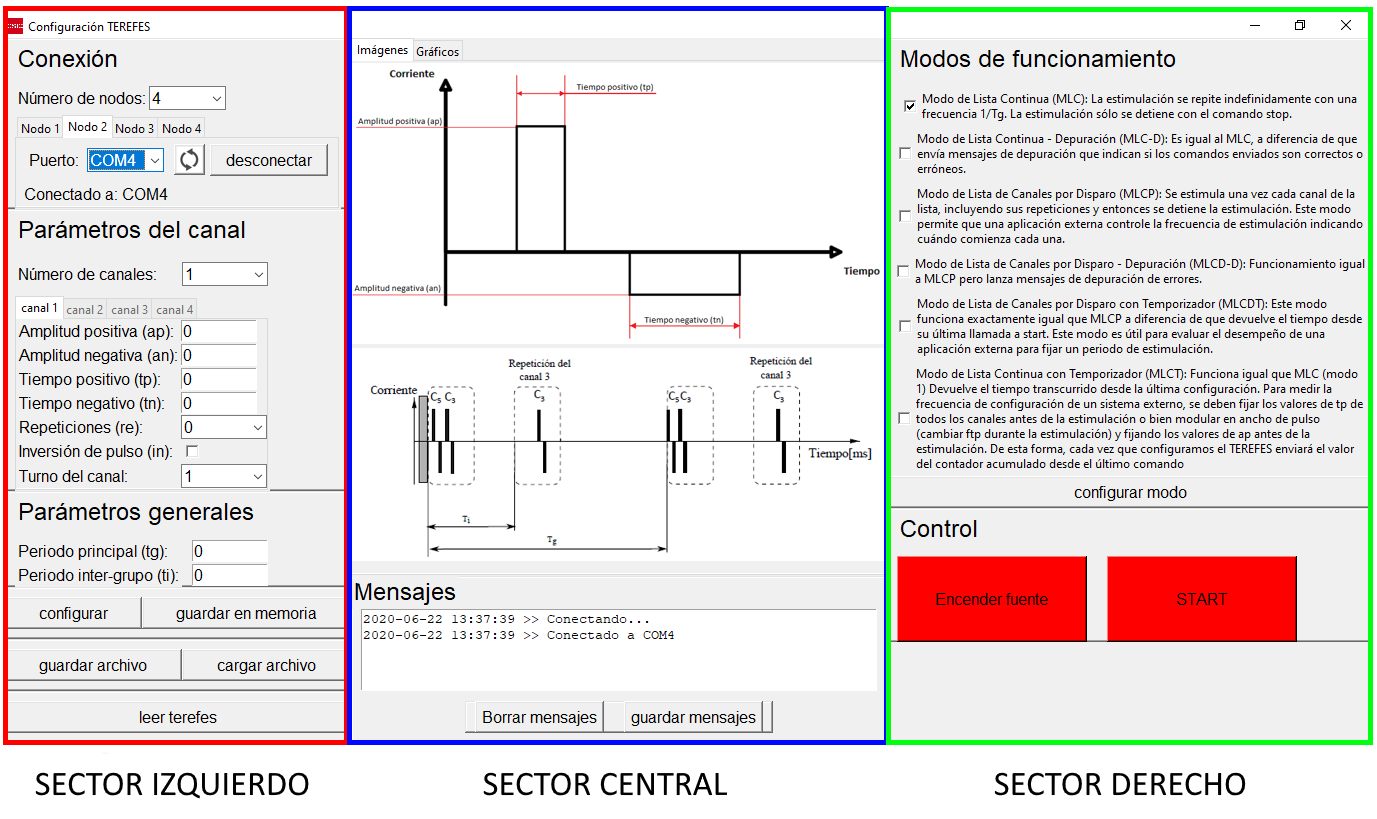
\includegraphics[scale=0.45]{interfaz}
  \caption{Interfaz gráfica de usuario para el control de la prótesis híbrida}.\label{fig:interfaz}
\end{figure}

El sector izquierdo se compone por los cuadros de conexión, parámetros del canal y parámetros generales del estimulador. El sector central se compone por las imágenes representativas de los parámetros anteriores, así como de un cuadro de texto que lanza mensajes informativos al usuario mientras utiliza la interfaz. Por último, el sector derecho se compone por los modos de funcionamiento y los botones de control de la fuente de corriente y la estimulación.


\subsection{Sector izquierdo: configuración de parámetros}
En este sector se encuentra en primer lugar el cuadro de conexión. El ordenador que hace uso de la interfaz debe conectarse por puerto serie virtual mediante Bluetooth al módulo de comunicación inalámbrica sparkfun silver descrito en el capítulo \ref{capitulo_2}. Para ello se sirve de los siguientes elementos:
\begin{itemize}
\item[•] \textbf{Número de nodos:} mediante una lista desplegable es posible seleccionar hasta cuatro nodos, es decir, electroestimuladores. Bajo esta lista hay cuatro pestañas, cada una corresponde a uno de los cuatro nodos que se pueden manejar con la interfaz. Para cada uno de ellos se pueden realizar las siguientes acciones:
\begin{itemize}
\item[o] \textbf{Botón de búsqueda de puertos:} es un botón cuadrado con dos flechas en su interior. Al pulsarlo, el ordenador busca todos los puertos serie asociados a algún dispositivo.
\item[o] \textbf{Lista de puertos:} a la izquierda del botón anterior hay una lista desplegable que contiene todos los puertos encontrados y mediante la cual se puede seleccionar el puerto al que están conectados el módulo Bluetooth y el ordenador.
\item[o] \textbf{Botón ``conectar'':} para establecer la conexión con el puerto seleccionado en la lista se debe pulsar este botón que se sitúa a la derecha de la lista de puertos.
\end{itemize}
\end{itemize}

Debajo del cuadro de conexión está el cuadro de parámetros del canal. En este cuadro se pueden visualizar los parámetros de configuración de cada canal del estimulador haciendo uso de los siguientes elementos:

\begin{itemize}
\item[•] \textbf{Número de canales:} en una lista desplegable se puede seleccionar el número de canales que se quieren utilizar y cuyo valor está comprendido entre 1 y 4.
\item[•] \textbf{Parámetros del canal:} Debajo de la lista de selección de número del canales se agrupan los parámetros de cada uno. Cada canal tiene sus parámetros en su correspondiente pestaña indicada por ``canal 1'', ``canal 2'', ``canal 3'' o ``canal 4'' según el caso. El usuario puede aquí modificar los valores de los parámetros de la siguiente forma:
\begin{itemize}
\item[o] \textbf{ap, an, tp, tn:} valores de amplitud de corriente y tiempo de pulso. Se introducen por teclado en el cuadro correspondiente.  
\item[o] \textbf{Repeticiones y turno:} indica las veces que se repite la estimulación del canal correspondiente y su turno de estimulación. Se selecciona el valor deseado de la lista desplegable.
\item[o] \textbf{Inversión:} indica si se invierte el primer pulso de corriente o no. Se marca o desmarca la casilla si se quiere tener esta inversión o no, respectivamente.
\end{itemize}           
\end{itemize}

El cuadro de parámetros generales permite editar los valores de las frecuencias inter pulso (tg) e intra pulso (ti) mediante entradas de texto por teclado.
\\
\\
Los demás elementos en este sector son botones los cuales realizan las siguientes acciones:
\begin{itemize}
\item[•] \textbf{Configurar:} tras pulsar este botón se recogen todos los valores de parámetros introducidos por el usuario y los envía al estimulador mediante el puerto serie seleccionado en el cuadro de conexión. Para ello, se hace uso de los comandos de configuración explicados en el capítulo \ref{capitulo_2} y que se implementan internamente en los métodos correspondientes en el código que conforma la interfaz de usuario.
\item[•] \textbf{Guardar en memoria:} este botón indica al estimulador que guarde en su memoria interna los valores de los parámetros que tiene configurados. 
Es importante mencionar que este botón no guarda en el estimulador los valores que hay visibles en la interfaz, para ello hay que configurar primero el estimulador con estos valores y después pulsar el botón ``guardar en memoria'' para que el estimulador los guarde.
\item[•] \textbf{Guardar archivo:} si se desea guardar en un archivo de configuración los parámetros que hay en la interfaz, se debe pulsar este botón. Al pulsarlo se pedirá al usuario el nombre del archivo de texto que contendrá los valores de los parámetros, así como dónde quiere guardarlo. Este archivo de configuración contiene el número de canales, los parámetros de cada canal y los parámetros generales.
\item[•] \textbf{Cargar archivo:} si se dispone de un archivo de configuración del estimulador, es posible cargar sus valores en la interfaz mediante este botón. Al pulsarlo se pedirá al usuario seleccionar el archivo de configuración. 
Esta acción solamente carga en la interfaz los valores del archivo de configuración, no los carga en el estimulador. Para ello es preciso pulsar el botón ``configurar''.
\item[•] \textbf{Leer estimulador:} este botón permite mostrar en la interfaz los valores de los parámetros que tiene configurados el estimulador. Tras pulsarlo, la interfaz comienza a leer los parámetros de cada canal y los generales mediante el puerto serie seleccionado en el cuadro de conexión y los muestra al usuario en la interfaz.
\end{itemize}

\subsection{Sector central: mensajes e imágenes informativos al usuario}
La parte superior de este sector, en la pestaña ``imágenes'', contiene dos imágenes que permiten visualizar qué representa cada parámetro del canal, así como los parámetros generales sobre esquemas de pulsos y trenes de pulsos de corriente.
\\
\\
Bajo las imágenes hay un cuadro de texto que muestra al usuario mensajes durante el manejo de la interfaz. Es útil para saber qué está ocurriendo tras pulsar cada botón así como para recibir mensajes de error en caso de que los hubiera. Cada mensaje viene precedido por la fecha y la hora en la que ocurre su evento asociado. Además, es posible borrar los menajes del cuadro de texto con el botón ``borrar mensajes'' al igual que se puede almacenarlos en un documento de texto con el botón ``guardar mensajes''.

\subsection{Sector derecho: modo de operación y control de estimulación}
En la parte superior de este sector se encuentra el cuadro de selección del modo de funcionamiento. Para seleccionar uno de los modos explicados en la interfaz se ha de marcar su casilla correspondiente. Después, para configurar dicho modo, se pulsa el botón ``configurar modo'' para que estimulador funcione acorde al mismo.
\\
\\
Por último, debajo de la selección del modo de funcionamiento está el cuadro de control con tres botones:

\begin{itemize}
\item[•] \textbf{Encender/apagar:} con este botón se puede encender o apagar la fuente de corriente del estimulador.
\item[•] \textbf{START/STOP:} este botón permite iniciar o detener la estimulación.
\end{itemize}



\section{Integración de sensores}


\section{Características especiales}
La interfaz tiene ciertas características que se explican a continuación y que permiten comprender mejor cómo funciona así como sus ventajas y limitaciones:

\begin{itemize}
\item[•] \textbf{Archivo configuración:} es posible cargar y guardar parámetros en un archivo de texto además de leer los parámetros ya cargados en el estimulador y mostrarlos en la interfaz. Para evitar cargar archivos de texto que no contienen parámetros de configuración en el formato que es capaz de leer la interfaz, estos archivos tienen en su primera línea la palabra ``miniFES''. Si al leer un archivo de texto la primera línea del mismo no contiene dicha palabra, no se cargará el archivo y avisará del error evitando así enviar al estimulador valores de parámetros incoherentes.
\item[•] \textbf{Entradas Acotadas:} se limitan los valores de parámetros que el usuario puede introducir en la interfaz. A continuación, se muestran los valores no admitidos:
\begin{itemize}
\item[a)] Valores negativos y fuera de los rangos de valores especificados en el capítulo \ref{capitulo_2}
\item[b)] Valores no numéricos
\item[c)] Valores con espacios delante o detrás: ``2'' ó ``2'' en vez de ``2'', por ejemplo
\item[d)] La entrada de texto está vacía.
\end{itemize}
Si el usuario introduce algún tipo de valor descrito anteriormente la interfaz lanzará el respectivo mensaje de error para corregirlo. Esta comprobación se efectúa cuando se configura el estimulador con los valores de la interfaz así como cuando se leen o se guardan los parámetros en un archivo de configuración.
\item[•] \textbf{Configuración rápida: } debido a que los parámetros se envían por puerto serie virtual vía Bluetooth, es necesario esperar cierto tiempo a que el mensaje llegue antes de enviar el siguiente por lo que enviar todos los parámetros cada vez que se configura el estimulador resulta muy lento. Se puede agilizar la configuración cuando solamente se modifican unos pocos parámetros manteniendo el resto iguales, es decir, sólo se envían los comandos de configuración de los parámetros que han cambiado respecto a la configuración anterior. Esto se aprecia en la tabla \ref{cuadro:configuracion_rapida} en la que se muestra que solamente los parámetros ``an'' y ``tg'' han cambiado respecto a la configuración anterior por lo que sólo se envían comandos para configurar ``an'' y ``tg''. De este modo se evita enviar comandos para reescribir ``ap'' y ``ti'' con los mismos valores y ahorrar tiempo de esta forma.

Además, en el modo 6 de funcionamiento los pulsos de corriente son cuadrados, es decir, ``ap'' y ``an'' son iguales, así como ``tp'' y ``tn'' por lo que el usuario solamente puede determinar el valor de ``ap'' y ``tp'' ya que ``an'' y ``tn'' tendrán el mismo valor respectivamente.

\begin{table}[!htb]
\centering
\begin{tabular}{| p{30mm} | p{30 mm} | p{30 mm} | p{30 mm} |}
\hline
\textbf{Parámetro} & \textbf{Valor inicial} & \textbf{Nuevo valor} & \textbf{Acción} \\ \hline
ap & 10 & 10 & Nada\\ \hline
an & 20 & 30 & Actualizar an \\ \hline
tg & 50 & 70 & Actualizar tg\\ \hline
ti & 50 & 50 & Nada\\ \hline
\end{tabular}\caption{Ejemplo de configuración rápida.}\label{cuadro:configuracion_rapida}
\end{table}

\item[•] \textbf{Estimulación segura:} la estimulación no se puede iniciar a no ser que la fuente de corriente esté encendida. Del mismo modo, si se apaga la fuente estando la estimulación iniciada, ésta terminará automáticamente. Por último, como medida de seguridad, cuando el usuario detiene la estimulación con su respectivo botón, no se hace ninguna comprobación respecto a las fuentes o el estado de la estimulación, ésta se detiene lo más rápido posible.

\item[•] \textbf{Threading: } La interfaz lleva a cabo tareas que duran un tiempo considerable, todas ellas relacionadas con la comunicación serie mediante Bluetooth. Si no se utiliza threading, tanto la interacción con la interfaz como las tareas que ésta realiza ocurren en un hilo principal. Esto quiere decir que, por ejemplo, al pulsar el botón ``configurar'' se envían los parámetros al estimulador y mientras esto ocurre el botón y toda la interfaz se quedan boqueados y no responderán hasta que termine la tarea de configurar el estimulador. Una solución (además de acelerar al máximo la comunicación por Bluetooth) es crear hilos independientes para tareas que necesitan tiempo y que pueden bloquear la interfaz. Esto sirve tanto para la transmisión y recepción de parámetros como el envío de comandos al estimulador para que realice determinadas tareas.

Las tareas para las que se crea su propio hilo son:

\begin{itemize}
\item[a.] \textbf{Configurar el estimulador:} se envían los parámetros necesarios, uno a uno, dejando entre cada transmisión un tiempo de 50$ms$ para dar tiempo al microcontrolador que los recibe a almacenarlos y procesarlos según el caso. Es la tarea que más tiempo requiere y motivo principal por el que se utiliza threading así como la característica de configuración rápida explicada en este apartado.
\item[b.] \textbf{Guardar parámetros en la EEPROM:} se trata de un comando corto y que lleva menos de dos segundos. Aun así, se considera como una tarea que puede bloquear la interfaz.
\item[c.] \textbf{Configurar modo:} misma situación que el caso anterior.
\item[d.] \textbf{Leer parámetros del estimulador:} es la tarea inversa a la configuración del estimulador: en vez de enviar parámetros al mismo es éste el que los envía a la interfaz. Tiene una duración similar a la tarea de configuración.
\item[e.] \textbf{Encender/apagar fuentes e iniciar/detener estimulación:} los comandos que necesita recibir el estimulador son cortos y su envío no requieren mucho tiempo, pero aun así pueden bloquear la interfaz brevemente.
\end{itemize}
\end{itemize}




















